\chapter{Modellazione dei Casi d'Uso}
\section{Attori e Casi d'Uso}
\begin{table}[!hbp]
	\centering
	\begin{tblr}{colspec=XX}
		\begin{minipage}[t]{\linewidth}
			\paragraph{Attori primari}
			\begin{itemize}
				\item UtenteNonRegistrato
				\item UtenteRegistrato
				\item Utente
				\item Amministratore
			\end{itemize}
		\end{minipage} &
		\begin{minipage}[t]{\linewidth}
			\paragraph{Attori secondari}
			\begin{itemize}
				\item SistemaGestioneAcquisti	
			\end{itemize}
		\end{minipage} \\
	\end{tblr}
\end{table}
\begin{table}[!hbp]
	\centering
	\begin{tblr}{colspec=XX}
		\begin{minipage}[t]{\linewidth}
			\paragraph{Casi d'uso}
			\begin{enumerate}
				\item Registrazione 
				\item Autenticazione
				\item RicercaEvento
				\item PubblicaEvento
				\item ConsultaInfromazioniEvento
				\item ConsultaCatalogoEventi
				\item PartecipazioneEvento
				\item AcquistoBiglietto
				\item ModificaDatiPersonali
				\item ConsultaStoricoBiglietti
				\item VisualizzaBiglietto
				\item ScaricaBiglietto
			\end{enumerate}
		\end{minipage} &
		\begin{minipage}[t]{\linewidth}
			\paragraph{Casi d'uso di inclusione}
			\begin{enumerate}
                \item ConsultaCatalogoEventi
			\end{enumerate}

		\end{minipage}
	\end{tblr}
\end{table}
\begin{table}[!ht]
\centering
\small
\begin{tblr}{
  colspec = {X[2,l] X[1.2,l] X[1,l] X[1.6,l] X[1.5,l]},
  hlines,
  row{1} = {font=\bfseries}
}
Caso d'uso & Attori Primari & Attori Secondari & Incl. / Ext. & Requisiti corrispondenti \\
Registrazione & UtenteNonRegistrato & -- & -- & \Req{rf}{01} \\
Aunteticazione & UtenteRegistrato & -- & -- & \Req{rf}{02} \\
RicercaEvento & UtenteRegistrato & -- & -- &\Req{rf}{08} \\
PubblicaEvento & Amministratore & -- & -- & \Req{rf}{06} \\
ConsultaInformazioniEvento & Amministratore & -- & Include: Consulta Catalogo Eventi & \Req{rf}{16}, \Req{rf}{17} \\
ConsultaCatalogoEventi & UtenteRegistrato & --  & \Req{rf}{07} \\
PartecipazioneEvento& Utente & -- & -- & \Req{rf}{14} \\
AcquistaBiglietto & Utente & SistemaGestioneAcquisti & Include: ConsultaCatalogoEventi & \Req{rf}{09} \\
ModificaDatiPersonali & Utente & -- & -- & \Req{rf}{5} \\
ConsultaStoricoBiglietti & Utente & -- & --  & \Req{rf}{04} \\
VisualizzaBiglietto & Utente & -- & -- & \Req{rf}{11} \\
ScaricaBiglietto & Utente & -- & -- & \Req{rf}{12} \\
\end{tblr}
\end{table}

\section{Diagramma dei Casi d'Uso}
\begin{table}[!ht]
\centering
	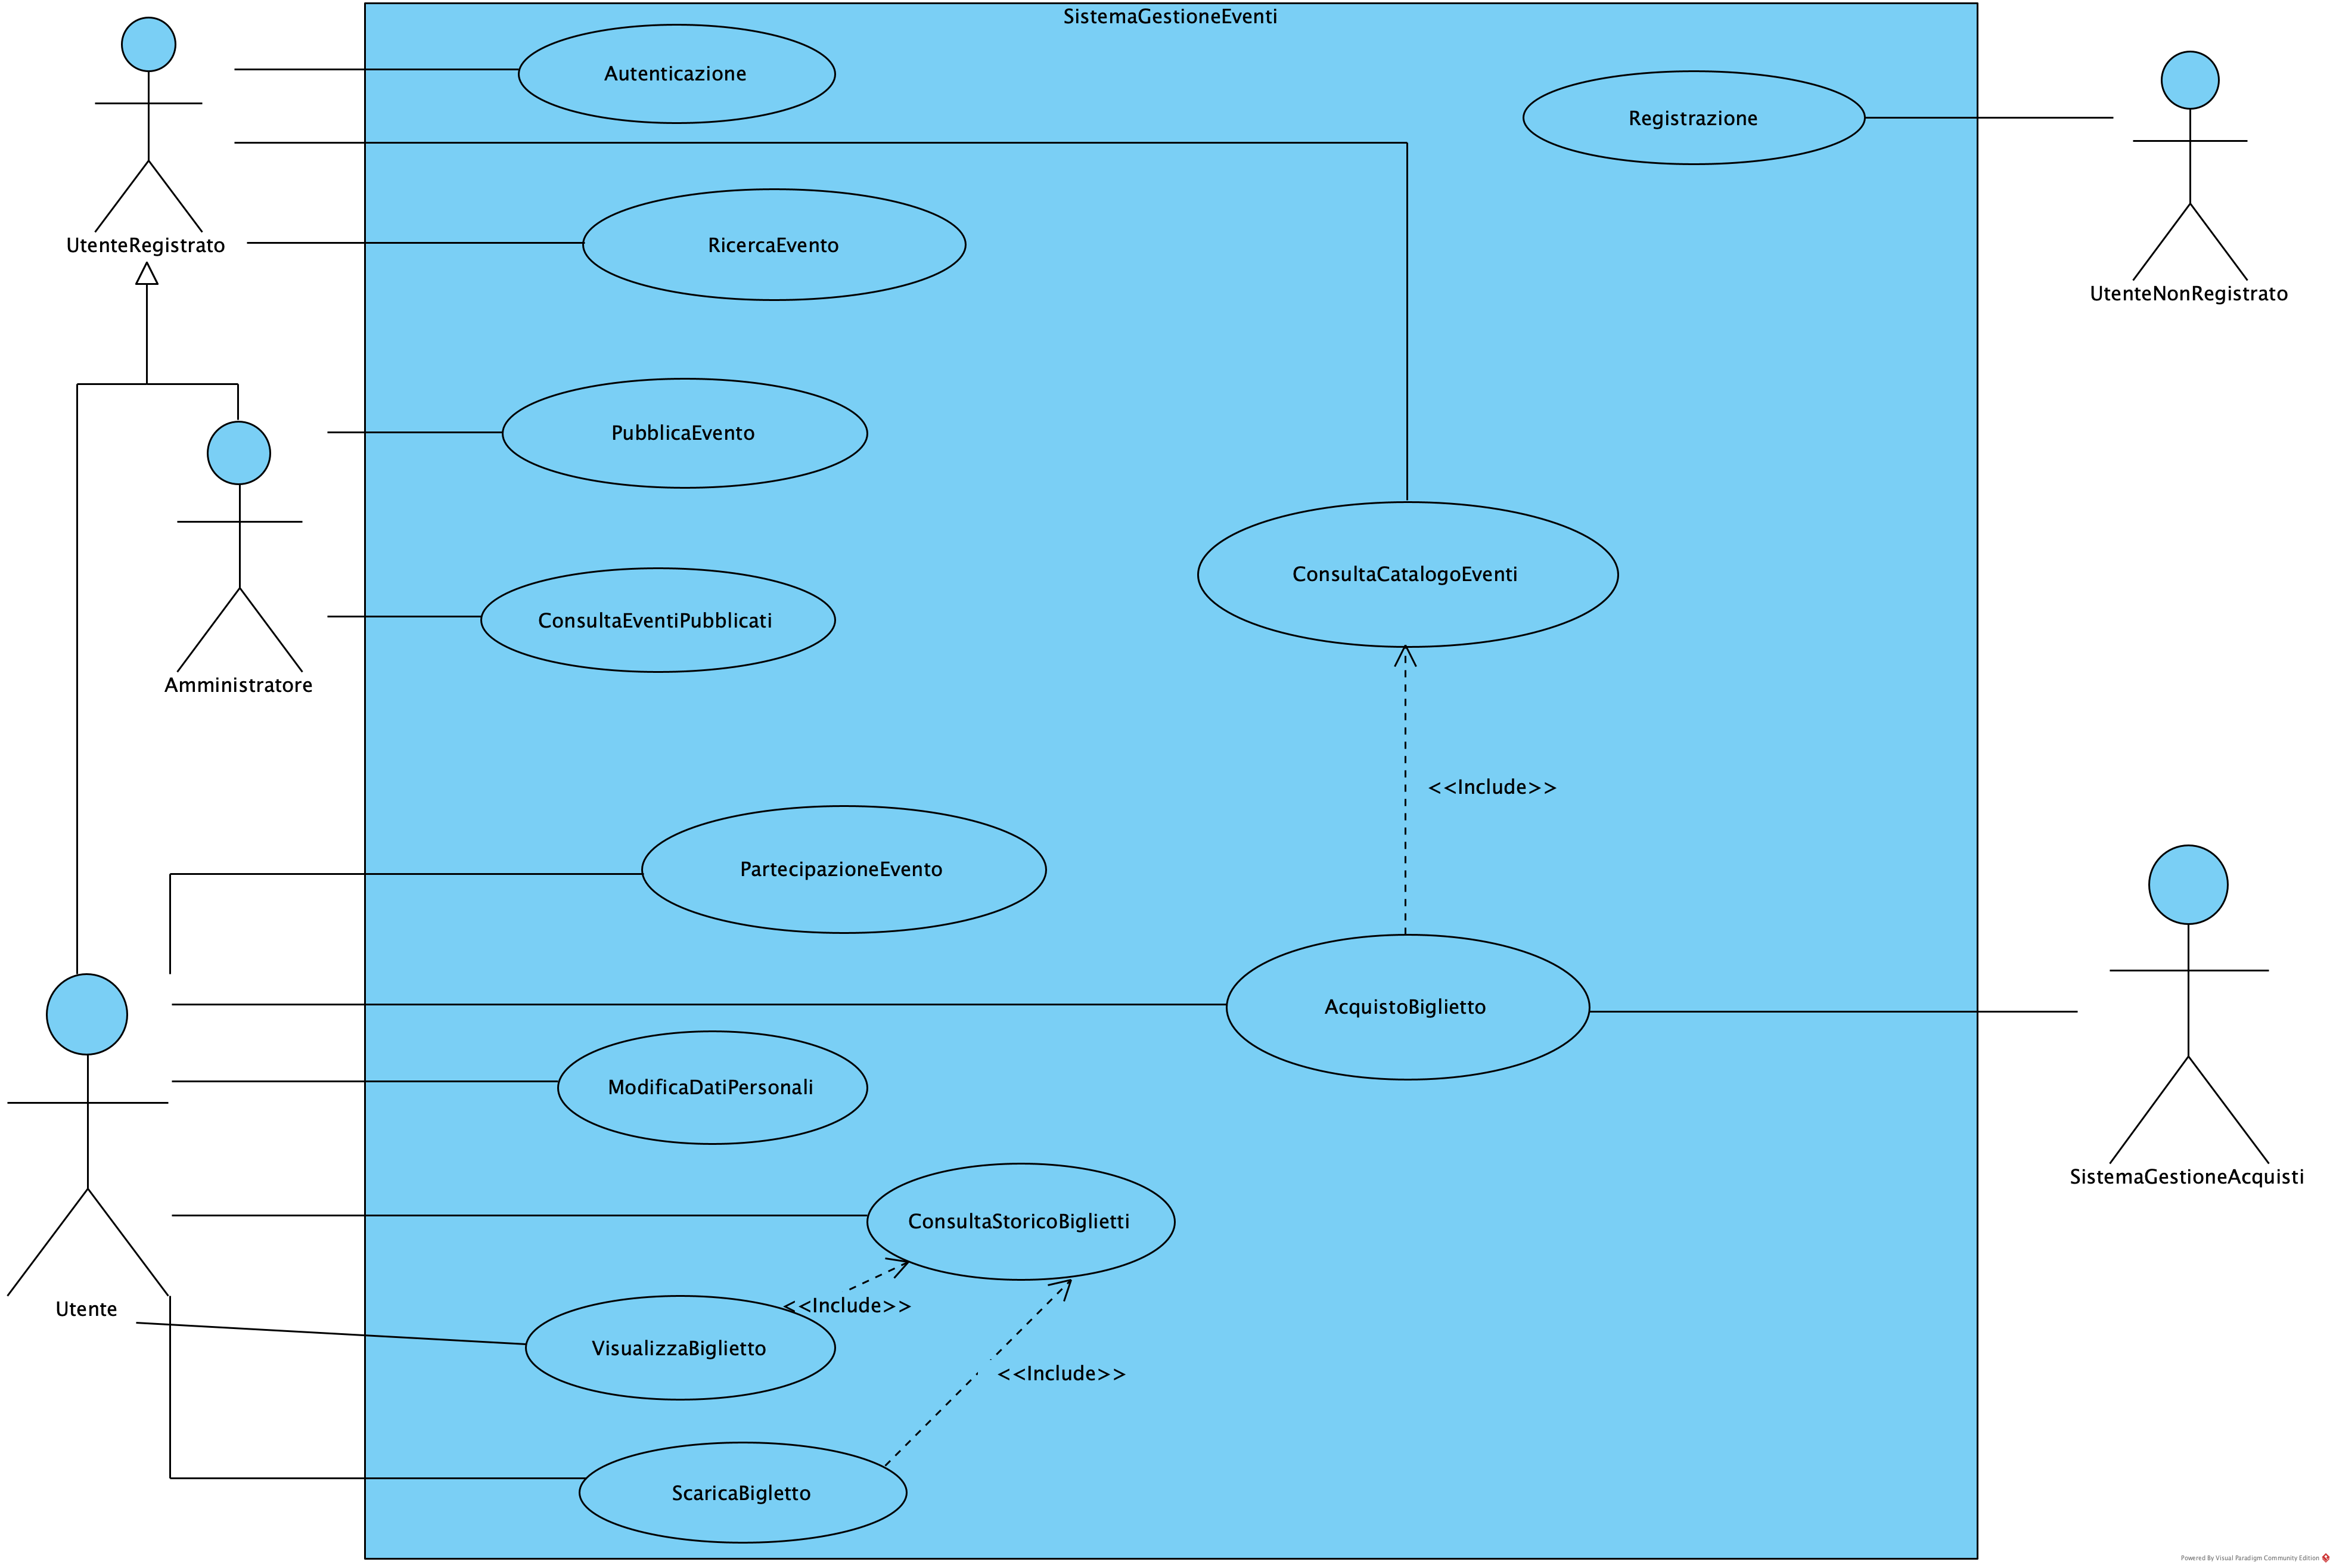
\includegraphics[width=\linewidth]{assets/casid'uso/Usd.png}
\end{table}	
\pagebreak
\section{Scenari}
\IncludeTable{capitoli/scenari/Registrazione}
\IncludeTable{capitoli/scenari/Autenticazione}
\IncludeTable{capitoli/scenari/ModificaDatiPersonali}
\IncludeTable{capitoli/scenari/ConsultaCatalogoEventi}
\IncludeTable{capitoli/scenari/RicercaEvento}
\IncludeTable{capitoli/scenari/VisualizzaBiglietto}
\IncludeTable{capitoli/scenari/ConsultaStoricoBiglietti}
\IncludeTable{capitoli/scenari/ScaricaBiglietto}
\IncludeTable{capitoli/scenari/AcquistaBiglietto}
\IncludeTable{capitoli/scenari/PubblicaEvento}
\IncludeTable{capitoli/scenari/PartecipazioneEvento}
\IncludeTable{capitoli/scenari/ConsultaInformazioniEvento}
\newpage
\section{Diagramma delle Classi}
Di seguito riportiamo il diagramma delle classi di analisi.
\begin{figure}[!ht]
	\centering
	%\includegraphics[width=0.8\linewidth]{assets/ClassDiagramAnalisi.png}
	\caption{Diagramma delle classi di analisi}
\end{figure}
